\documentclass[letter]{article}

\usepackage{color}

\usepackage{amsmath}
\usepackage{algorithm}
\usepackage[noend]{algpseudocode}
\usepackage{graphicx}

\begin{document}

\title{The Metropolis Parallel Sort Algorithm}
\author{Jamshid  Farzidayeri, Graham West, JJ Lay}
\date{Wednesday, January 16, 2019}

\maketitle

% \section{Algorithm}
% 
% \begin{algorithm}
% \caption{Parallel Sort}
% \begin{algorithmic}[1]
% \Procedure{ParallelSort}{}
%   \State $N \gets \text{Number of } numbers$
%   \State $n \gets \text{Number of MPI } nodes$
%   \State Send $N/n$ numbers to each node\;
%   \State $Run \gets \text{True}$
%   \While{(Run)}
%      \State Each node sorts its values
%      \State Swap some data here
%      \If{(Some test)}
%         \State $Run \gets \text{False}$
%      \EndIf
%   \EndWhile
% \EndProcedure
% \end{algorithmic}
% \end{algorithm}


\section{Algorithm}

\begin{description}
\item[1.]{Distribute data to each node}
\item[2.]{Each node sorts its data}
\end{description}
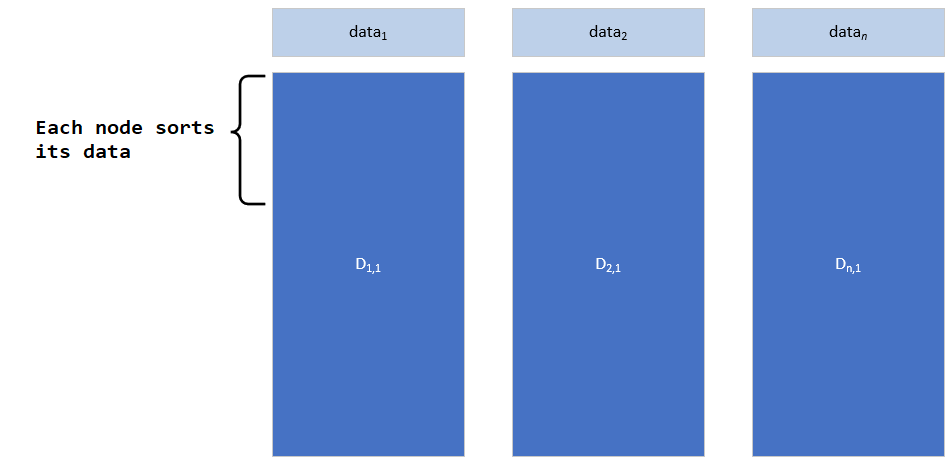
\includegraphics[width=0.7\textwidth]{images/Capture0.PNG}

\begin{description}
\item[3.]{Data on each node is divided into two sections of sizes $N \times r$ and $N \times (1-r)$ (where $r$ is a ratio selected by the user and $N$ is the number of values to be sorted)}
\end{description}
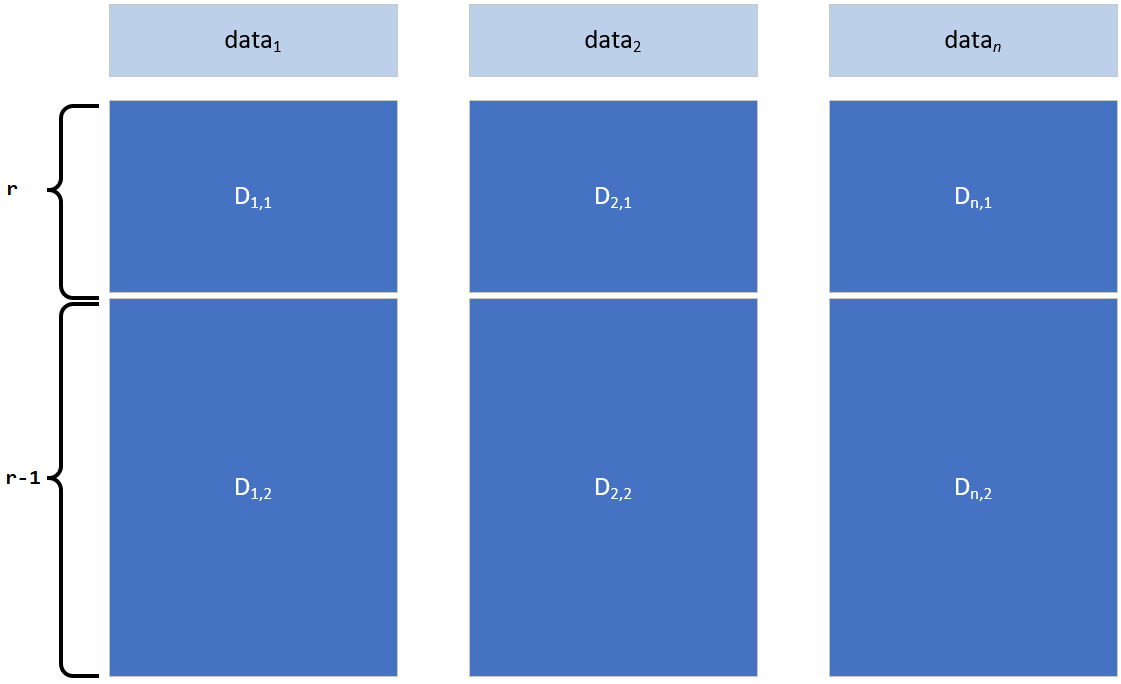
\includegraphics[width=0.7\textwidth]{images/Capture1.PNG}

\newpage

\begin{description}
\item[4.]{For the first $n-1$ nodes, the largest $(r-1)/N$ data is marked for transmission}
\end{description}
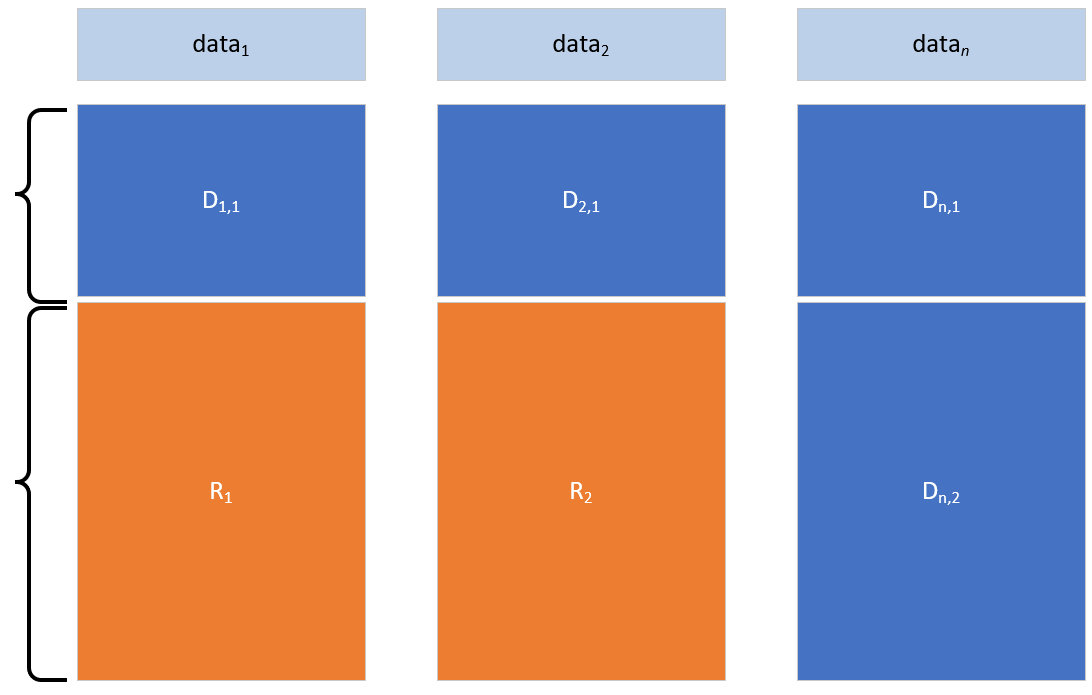
\includegraphics[width=0.7\textwidth]{images/Capture2.PNG}

\begin{description}
\item[5.]{The largest values from node $j$ is shifted to the front of the list on node $j+1$}
\end{description}
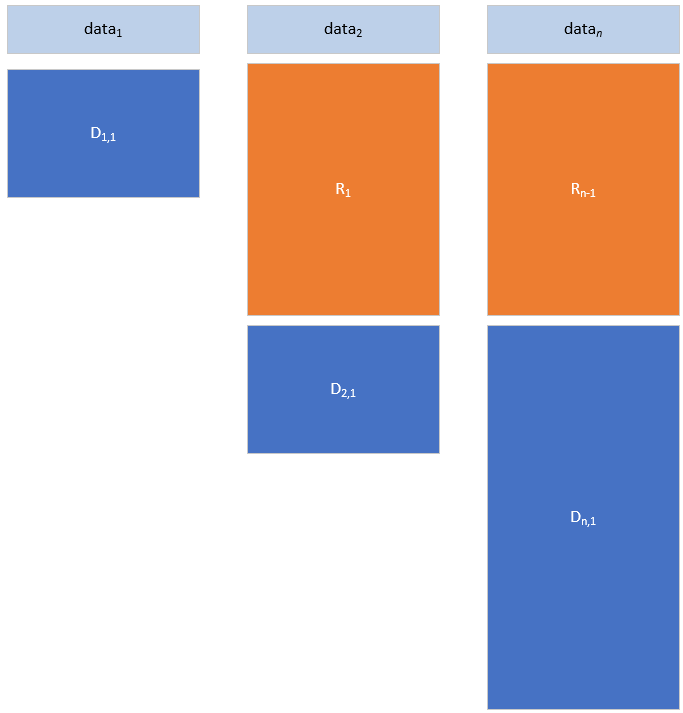
\includegraphics[width=0.7\textwidth]{images/Capture3.PNG}

\newpage

\begin{description}
\item[6.]{Each node sorts its new data set}
\end{description}
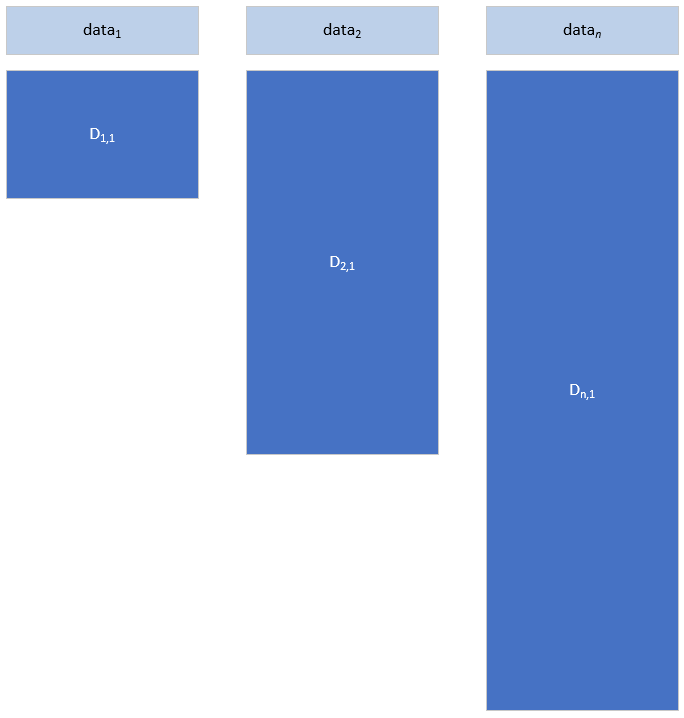
\includegraphics[width=0.7\textwidth]{images/Capture4.PNG}

\begin{description}
\item[7.]{For the last $n-1$ nodes, the smallest $N \times (r-1)$ data is marked for transmission}
\end{description}
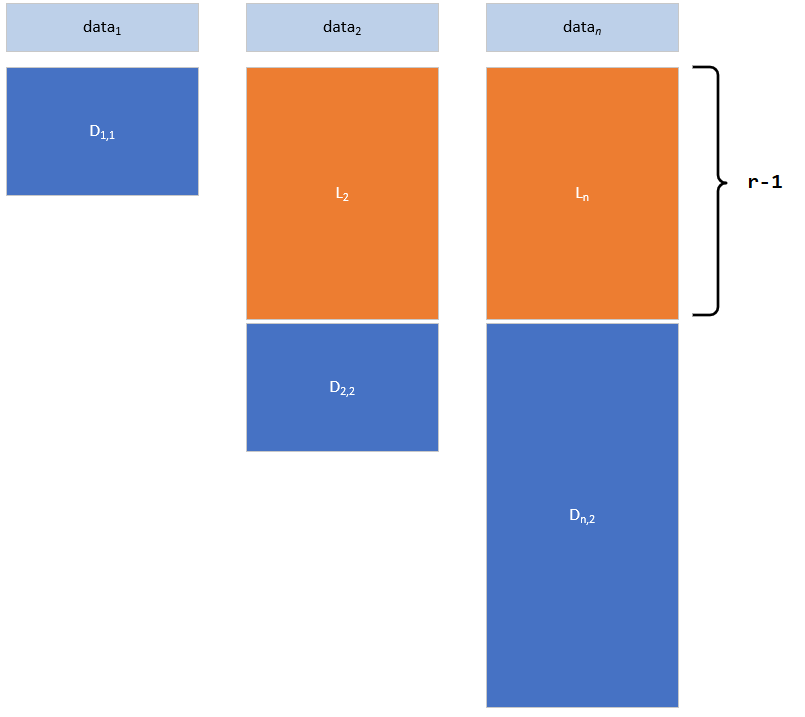
\includegraphics[width=0.7\textwidth]{images/Capture5.PNG}

\newpage

\begin{description}
\item[8.]{The smallest values from node $j$ is shifted to back of the list on node $j-1$}
\end{description}
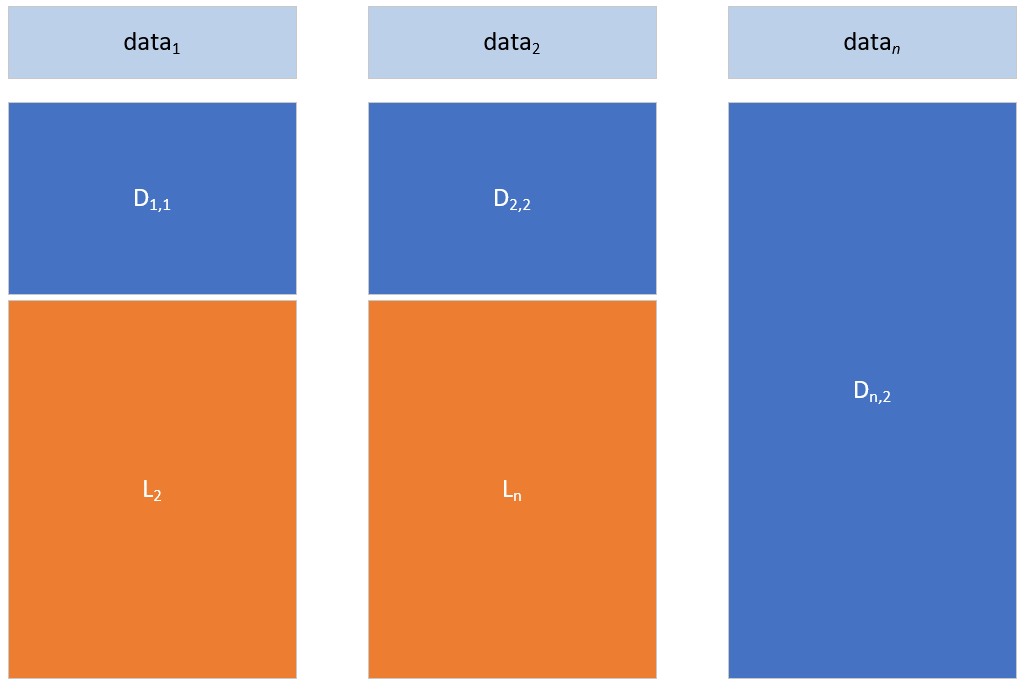
\includegraphics[width=0.7\textwidth]{images/Capture6.PNG}

\begin{description}
\item[9.]{Each node sorts its data}
\end{description}
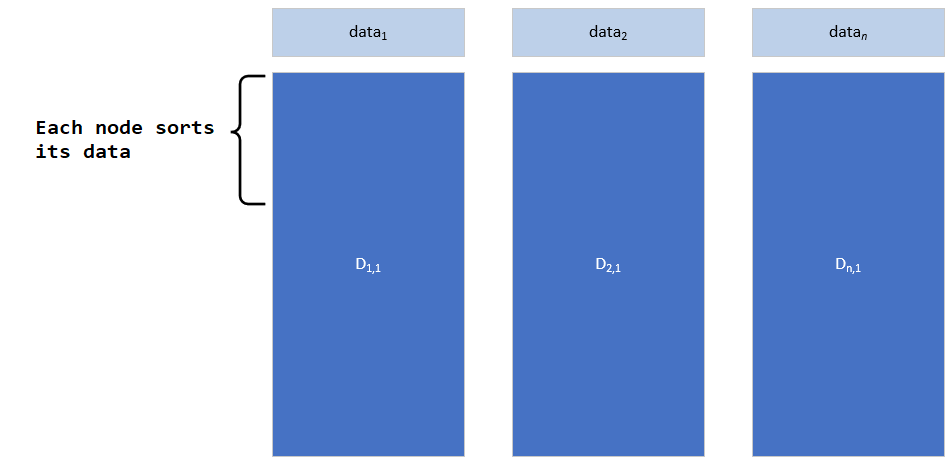
\includegraphics[width=0.7\textwidth]{images/Capture0.PNG}

\begin{description}
\item[10.]{Nodes exchange max values}
\item[11.]{If any node $j$ has a min value less than the max value of a node less than $j$, then loop to step 3}
\item[12.]{Nodes return results to node 0}
\item[13.]{Node 0 exports final results}
\end{description}

\end{document}
